\documentclass{article}

\usepackage{fullpage}

\usepackage{multicol}
\usepackage{graphicx}
\usepackage{svn-multi}
\usepackage{hyperref}


\hyphenation{O-pen-Earth}

% subversion
\svnidlong
{$HeadURL: https://svn.oss.deltares.nl/repos/openearthtools/trunk/latex/svn_manual/svn_manual.tex $}
{$LastChangedDate: 2018-01-10 02:43:24 -0800 (Wed, 10 Jan 2018) $}
{$LastChangedRevision: 14083 $}
{$LastChangedBy: heijer $}
\svnid{$Id: svn_manual.tex 14083 2018-01-10 10:43:24Z heijer $}
\svnRegisterAuthor{heijer}{Kees den Heijer}
\newcommand{\svnUrl}{https://svn.oss.deltares.nl/repos/openearthtools/trunk/}
\newcommand{\svnDir}{openearthtools}

\hypersetup{
linkcolor=blue, % color of internal links
citecolor=blue, % color of links to bibliography
filecolor=blue, % color of file links
urlcolor=blue % color of external links
}

\parindent 0pt
\usepackage[english]{babel} % select language

\graphicspath{{figures/}}

\author{\svnFullAuthor{\svnauthor}}
\title{Manual on using subversion (SVN)}
\date{\svntoday}

\begin{document}

%\makememoHeader
%------------------------------------------------------------------------------
%\tableofcontents

\maketitle

% subversion
\svnidlong
{$HeadURL: https://svn.oss.deltares.nl/repos/openearthtools/trunk/latex/svn_manual/contents/tutorial_svn.tex $}
{$LastChangedDate: 2018-07-16 12:22:21 -0700 (Mon, 16 Jul 2018) $}
{$LastChangedRevision: 14493 $}
{$LastChangedBy: heijer $}
\svnid{$Id: tutorial_svn.tex 14493 2018-07-16 19:22:21Z heijer $}

This document elaborates on working with Subversion, either via your web browser, TortoiseSVN or command line.
For some suggestions about the structuring of a repository is referred to \url{https://publicwiki.deltares.nl/display/OET/Raw+data+repository+structuring}.

\section{Browse}
Go to the url of the repository, e.g. \url{\svnUrl}.
This allows you to browse through the directory structure of the repository and view individual files (text files only) or download them.
TortoiseSVN includes a \emph{repo-browser} that provides a similar overview of the directory structure and files.

\section{Installation}

To be able to also contribute to repositories, subversion client software needs to be installed on your machine.
 
\begin {itemize}

\item TortoiseSVN (\url{https://tortoisesvn.net/downloads.html}) is recommended for Windows.
\begin{itemize}

\item It is recommended to enable the option \emph{command line tools} during the installation of TortoiseSVN.
By default the option is disabled, as indicated in the figure below.
\newline 

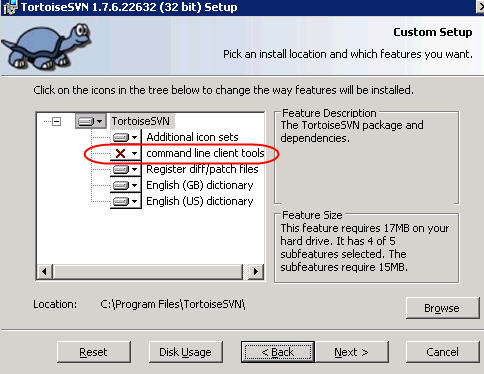
\includegraphics [width=242px] {command_line_tools}
\newline

\end{itemize}
\item SmartSVN (\url{https://www.smartsvn.com/download/}) is recommended for OS X, if you prefer to work with a user interface.
\item Command line client tools are available for all platforms. On linux you can install it with:
\begin{itemize}
\item \texttt{sudo apt install subversion} (Ubuntu/Debian)
\item \texttt{sudo yum install subversion} (Centos)
\end{itemize}
\end {itemize}

The right hand side of this tutorial gives some useful command line client commands.

\section{Checkout}
When making a \emph{checkout}, one makes a local copy of the folders and files on his or her computer. 
Be careful, do not try to make a local copy of the whole repository since it can easily grow beyond the storage capacity of you computer.

\begin {multicols}{2}
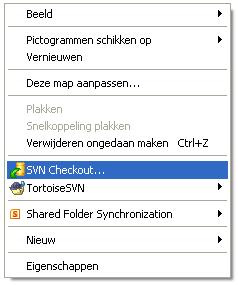
\includegraphics [width=150px]{checkout_blue}
\columnbreak

\texttt{svn checkout --username=<USERNAME>} \\
\texttt{\svnUrl{}}
\texttt{\svnDir{}}

\emph{PLEASE NOTE: this is the default checkout command which is certainly not recommended in case of large data repositories since the data volume will soon grow beyond the storage capacity of your computer.}
\end{multicols}

\begin {multicols}{2}
\begin{itemize}
\item \emph{Fully recursive:} Checkout the entire tree, including all child folders and sub-folders. \emph{PLEASE NOTE: this is the default checkout command which is certainly not recommended in case of large data repositories since the data volume will soon grown beyond the storage capacity of your computer.}
\end {itemize}
\columnbreak
\texttt{svn checkout --username=<USERNAME>} \\
\texttt{--depth infinity } \\
\texttt{\svnUrl{}}
\texttt{\svnDir{}}
\end{multicols}

\begin {multicols}{2}
\begin {itemize}
\item \emph{Immediate children, including folders:} Checkout the specified directory, including all files and child folders, but do not populate the child folders.
\end {itemize}
\columnbreak
\texttt{svn checkout --username=<USERNAME>} \\
\texttt{--depth immediates } \\
\texttt{\svnUrl{}}
\texttt{\svnDir{}}
\end {multicols}

\begin {multicols}{2}
\begin {itemize}
\item \emph {Only file children:} Checkout the specified directory, including all files but do not checkout any child folders.
\end {itemize}
\columnbreak
\texttt{svn checkout --username=<USERNAME>} \\
\texttt{--depth files } \\
\texttt{\svnUrl{}}
\texttt{\svnDir{}}
\end {multicols}

\begin {multicols}{2}
\begin {itemize}
\item \emph {Only this item:} Checkout the directory only. Do not populate it with files or child folders.
\end {itemize}
\columnbreak
\texttt{svn checkout --username=<USERNAME>} \\
\texttt{--depth empty } \\
\texttt{\svnUrl{}}
\texttt{\svnDir{}}
\end {multicols}

\section{Important Actions}
The two most important commands are \emph{SVN Update} and \emph{SVN Commit}. It is very important to use \emph{SVN Update} regularly, but especially when you start working on a certain file/directory. If this command is not used, it might happen that someone else in the meantime has been updating the file/directory; which means that you are working with an older version of this file/directory. On the other hand, it is very important to use \emph{SVN Commit} at the end of the day. This command uploads the files you have been working on, so all others will be able to work with the most recent versions. When you use \emph{SVN Commit}, you should always write a log message in English. This message gives everyone the possibility to see what is changed. You can either commit one file or folder, or the entire tree. 

\section{Update}
\begin{multicols}{2}
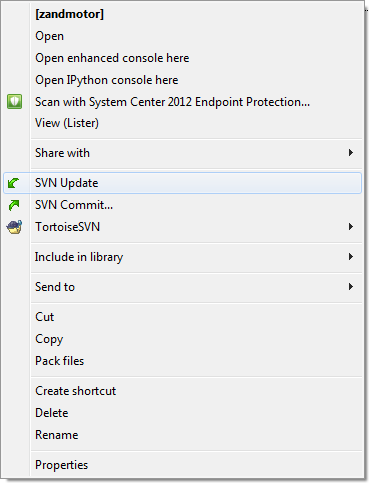
\includegraphics[width=150px]{update_selected}
\columnbreak
\newline Assuming that you are in the path of your checkout, use:
\begin{verbatim}
svn up
\end{verbatim}
or
\begin{verbatim}
svn update
\end{verbatim}
\end{multicols}

\section{Commit}
By committing, you are performing the actual uploading of your local modifications, additions or deletions to the server.

\begin{multicols}{2}
Right-click on the file or folder that you want to commit and select \emph{SVN Commit} from the list. 
\newline
\newline
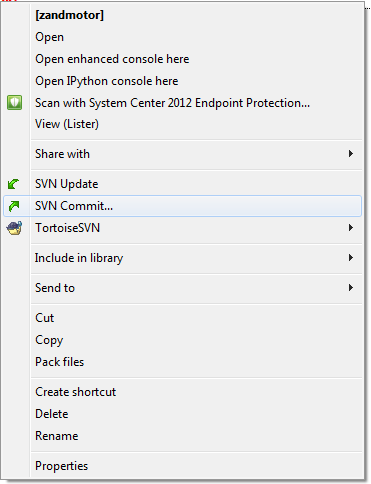
\includegraphics[width=200px]{commit_selected}
\columnbreak %columnbreak heeft geen invloed?
\newline To get an overview of the files that you are about to commit, use:
\begin{verbatim}
svn st
\end{verbatim}
or
\begin{verbatim}
svn status
\end{verbatim}
The actual commit action is performed by the following command:
\begin{verbatim}
svn ci -m"write your custom concise 
summary of your contribution here"
\end{verbatim}
Make sure that you provide a useful but concise message between the quotes (in English). 
\end{multicols}

\begin{multicols}{2}
A window pops up that provides you with an overview of the items that you are about to commit. Make sure that you fill in a useful but concise message in the message window (in English). If you are doing similar commits multiple times, it is useful to make use of the \emph{Recent messages} to save the number of key strokes. Only the files that are selected (tick box left) will be send to the server. 
\columnbreak
\ \
\newline %Hoe dit normaal op te lossen?
\newline
\newline
\ \ 
\end{multicols}
\begin{multicols}{2}
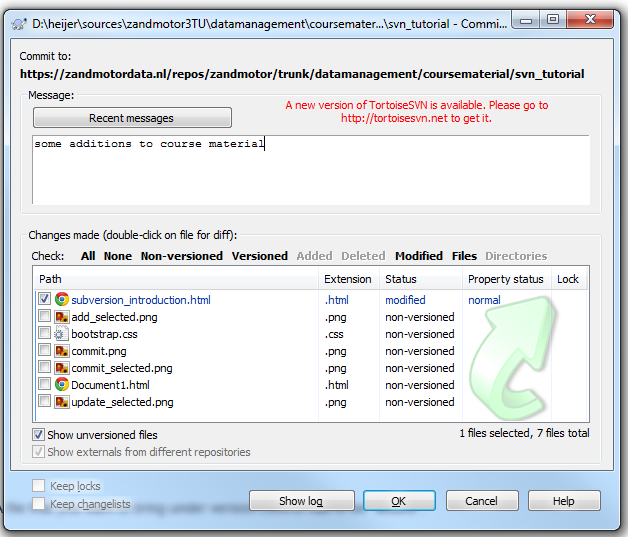
\includegraphics[width=220px]{commit}
\end{multicols}
\begin{multicols}{2}
Ticking the box of a \emph{non-versioned} file has the same effect as \emph{adding} a file. 
\ \ 
\newline
\ \
\end{multicols}

\section{Add}
A newly created file in your local file system is by default not under version control. A file that you want to bring under version control has to be \emph{added}, meaning that you nominate the file to be uploaded on the next commit. 

\begin{multicols}{2}
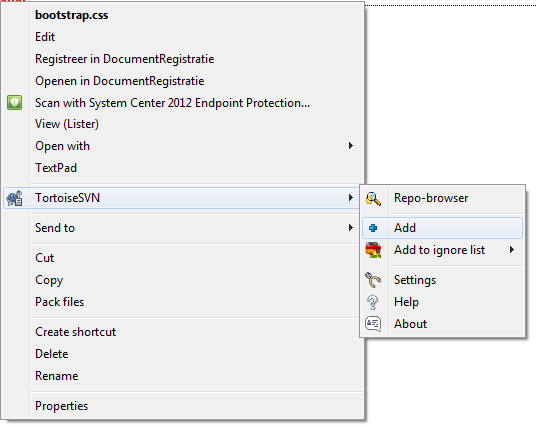
\includegraphics[width=200px]{add_selected}
\columnbreak
\begin{verbatim}
svn add FILENAME
\end{verbatim}

\end{multicols}
\newpage

\section{Delete}
Locally deleting a file does not automatically mean that it is also deleted on the server. If the server does not know that the file should be deleted, it will see the file as locally missing, and will restore the file on the next update. By using the \emph{Delete} option of your SVN client, the file will be deleted locally and remember that it has to be deleted on the server during the next commit action. 

\begin{multicols}{2}
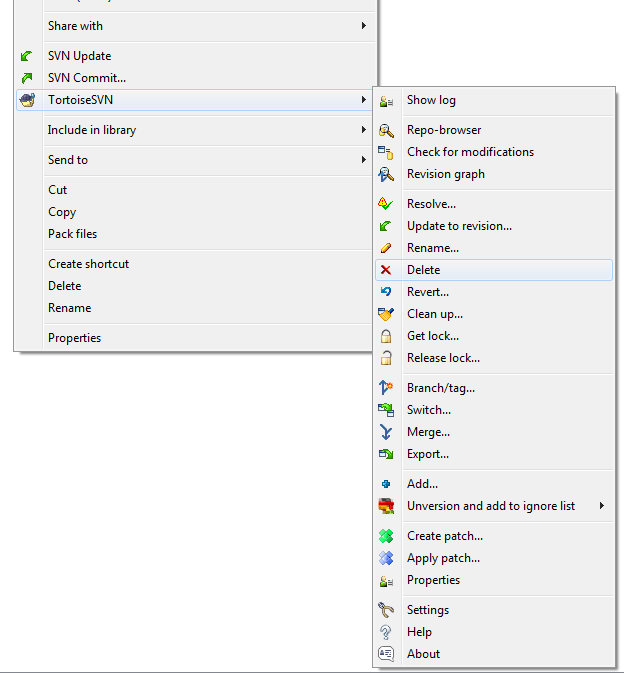
\includegraphics[width=200px]{delete_selected}
\columnbreak
\begin{verbatim}
svn rm FILENAME
\end{verbatim}

\end{multicols}

\section{Log}
To get an overview of the activity on the server, the SVN log can be used. 

\begin{multicols}{2}
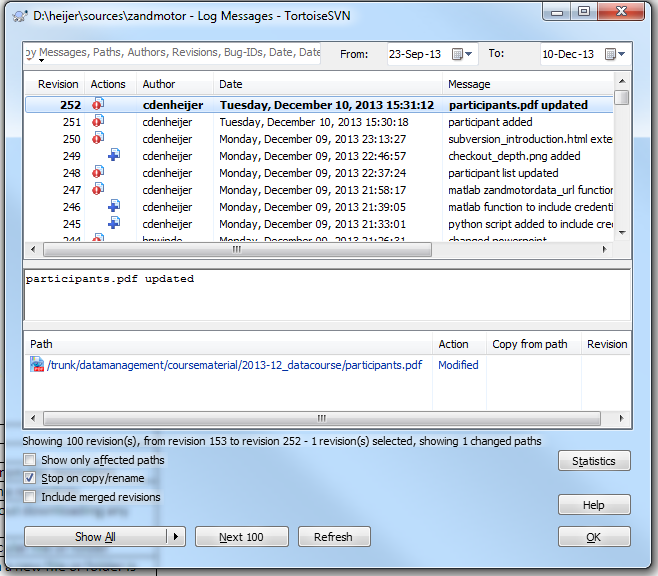
\includegraphics[width=220px]{show_log}
\columnbreak
\newline The following command provides you with all the log messages, which can be a long list: 
\begin{verbatim}
svn log
\end{verbatim}
To limit the number of records, you can limit them to e.g. 10 like this:
\begin{verbatim}
svn log -1 10
\end{verbatim}
\end{multicols}



%\section{Referenties}
%\bibliographystyle{deltares_chicago_like} % set style
%\bibliography{../../library/bibliography/journal-titles,../../library/bibliography/bibliography} % relative reference to bibliography file  

%%------------------------------------------------------------------------------
\end{document}